%% build: latexmk -pdf -pvc prez.tex

\documentclass[dvipsnames]{beamer}
\usetheme{Madrid}

%% kill footline
\setbeamertemplate{footline}[frame number]{}
\setbeamertemplate{navigation symbols}{}
\setbeamertemplate{footline}{}

%% bibliography
\bibliographystyle{alpha}
\setbeamerfont{bibliography item}{size=\footnotesize}
\setbeamerfont{bibliography entry author}{size=\footnotesize}
\setbeamerfont{bibliography entry title}{size=\footnotesize}
\setbeamerfont{bibliography entry location}{size=\footnotesize}
\setbeamerfont{bibliography entry note}{size=\footnotesize}
\setbeamertemplate{bibliography item}{}

%% kill ball enumeration
\setbeamertemplate{enumerate items}[circle]
\setbeamertemplate{section in toc}[circle]

%% kill block shadows
\setbeamertemplate{blocks}[rounded][shadow=false]
\setbeamertemplate{title page}[default][colsep=-4bp,rounded=true]

%% kill ball itemize
\setbeamertemplate{itemize items}[circle]

%% --------------------------------------------------------------------------------

\usepackage[utf8]{inputenc}
%% \usepackage[hidelinks]{hyperref}
\usepackage{amsmath}
\usepackage{cite}
\usepackage{amsthm}
\usepackage{amssymb}
\usepackage{amsfonts}
\usepackage{mathpartir}
\usepackage{scalerel}
\usepackage{stmaryrd}
\usepackage{bm}
\usepackage{graphicx}

%% --------------------------------------------------------------------------------

%% HoTT style composition
\makeatletter
\DeclareRobustCommand{\sqcdot}{\mathbin{\mathpalette\morphic@sqcdot\relax}}
\newcommand{\morphic@sqcdot}[2]{%
  \sbox\z@{$\m@th#1\centerdot$}%
  \ht\z@=.33333\ht\z@
  \vcenter{\box\z@}%
}
\makeatother

\newcommand{\mi}[1]{\mathit{#1}}
\newcommand{\ms}[1]{\mathsf{#1}}
\newcommand{\mbb}[1]{\mathbb{#1}}
\newcommand{\mbf}[1]{\mathbf{#1}}
\newcommand{\bs}[1]{\boldsymbol{#1}}
\newcommand{\ap}{\ms{ap}}
\newcommand{\apd}{\ms{apd}}
\newcommand{\tr}{\ms{tr}}
\newcommand{\happly}{\ms{happly}}
\newcommand{\funext}{\ms{funext}}
\newcommand{\toind}{\to^{\ms{int}}}

\newcommand{\Tys}{\ms{Ty_{sig}}}
\newcommand{\Tms}{\ms{Tm_{sig}}}
\newcommand{\Us}{\ms{U_{sig}}}
\newcommand{\Els}{\ms{El_{sig}}}

\newcommand{\Ix}{\mi{Ix}}

\newcommand{\zero}{\ms{zero}}
\newcommand{\suc}{\ms{suc}}
\newcommand{\J}{\ms{J}}
\newcommand{\UIP}{\ms{UIP}}

\newcommand{\refl}{\mathsf{refl}}
\newcommand{\reflect}{\mathsf{reflect}}
\newcommand{\Reflect}{\mathsf{Reflect}}
\newcommand{\id}{\mathsf{id}}
\newcommand{\Con}{\mathsf{Con}}
\newcommand{\Sub}{\mathsf{Sub}}
\newcommand{\Tm}{\mathsf{Tm}}
\newcommand{\Ty}{\mathsf{Ty}}
\newcommand{\U}{\mathsf{U}}
\newcommand{\El}{\mathsf{El}}
\newcommand{\Id}{\mathsf{Id}}
\newcommand{\ID}{\mathsf{ID}}
\newcommand{\proj}{\mathsf{proj}}
\renewcommand{\tt}{\mathsf{tt}}
\newcommand{\blank}{\mathord{\hspace{1pt}\text{--}\hspace{1pt}}}
\newcommand{\ra}{\rightarrow}
\newcommand{\Set}{\mathsf{Set}}
\newcommand{\Sort}{\mathsf{Sort}}

\newcommand{\Lift}{\Uparrow}
\newcommand{\ToS}{\mathsf{ToS}}
\newcommand{\ext}{\triangleright}
\newcommand{\emptycon}{\scaleobj{.75}\bullet}

\newcommand{\Pii}{\Pi}
\newcommand{\funi}{\Rightarrow}
\newcommand{\appi}{\mathsf{app}}
\newcommand{\lami}{\mathsf{lam}}

\newcommand{\fune}{\Rightarrow^{\ms{Ext}}}
\newcommand{\Pie}{\Pi^{\mathsf{Ext}}}
\newcommand{\appe}{\mathsf{app^{Ext}}}
\newcommand{\lame}{\mathsf{lam^{Ext}}}
\newcommand{\toe}{\to^{\ms{Ext}}}
\newcommand{\arre}{\Rightarrow^{\mathsf{Ext}}}
\newcommand{\lambdae}{\lambda^{\ms{Ext}}}

\newcommand{\Piinf}{\Pi^{\mathsf{ext}}}
\newcommand{\appinf}{\mathsf{app^{ext}}}
\newcommand{\laminf}{\mathsf{lam^{ext}}}
\newcommand{\laminfprime}{\mathsf{lam^{ext'}}}
\newcommand{\toinf}{\to^{\ms{ext}}}
\newcommand{\lambdainf}{\lambda^{\ms{ext}}}
\newcommand{\arrinf}{\Rightarrow^{\mathsf{ext}}}
\newcommand{\bPiinf}{\bs{\Piinf}}

\newcommand{\appitt}{\mathop{{\scriptstyle @}}}
\newcommand{\Refl}{\mathsf{Refl}}
\newcommand{\IdU}{\mathsf{IdU}}
\newcommand{\ReflU}{\mathsf{ReflU}}
\newcommand{\Sig}{\mathsf{Sig}}
\newcommand{\ToSSig}{\mathsf{ToSSig}}
\newcommand{\Subtype}{\mathsf{Subtype}}
\newcommand{\subtype}{\mathsf{subtype}}
\newcommand{\NatSig}{\mathsf{NatSig}}
\newcommand{\Sg}{\Sigma}
\newcommand{\flcwf}{\mathsf{flcwf}}
\newcommand{\SigTy}{\mathsf{SigTy}}
\newcommand{\SigTm}{\mathsf{SigTm}}
\newcommand{\SigU}{\mathsf{SigU}}
\newcommand{\tm}{\ms{tm}}
\newcommand{\ty}{\ms{ty}}

\newcommand{\Kfam}{\mathsf{K}}
\newcommand{\lamK}{\mathsf{lam}_{\K}}
\newcommand{\appK}{\mathsf{app}_{\K}}

\newcommand{\p}{\mathsf{p}}
\newcommand{\q}{\mathsf{q}}
\newcommand{\K}{\mathsf{K}}
\newcommand{\A}{\mathsf{A}}
\newcommand{\D}{\mathsf{D}}
\renewcommand{\S}{\mathsf{S}}
\newcommand{\arri}{\Rightarrow}
\newcommand{\syn}{\mathsf{syn}}
\newcommand{\SynSig}{\mathsf{SynSig}}
\newcommand{\bCon}{\bs{\Con}}
\newcommand{\bTy}{\bs{\Ty}}
\newcommand{\bSub}{\bs{\Sub}}
\newcommand{\bTm}{\bs{\Tm}}
\newcommand{\bGamma}{\bs{\Gamma}}
\newcommand{\bDelta}{\bs{\Delta}}
\newcommand{\bsigma}{\bs{\sigma}}
\newcommand{\bdelta}{\bs{\delta}}
\newcommand{\bepsilon}{\bs{\epsilon}}
\newcommand{\bt}{\bs{t}}
\newcommand{\bu}{\bs{u}}
\newcommand{\bA}{\bs{A}}
\newcommand{\ba}{\bs{a}}
\newcommand{\bb}{\bs{b}}
\newcommand{\bB}{\bs{B}}
\newcommand{\bid}{\bs{\id}}
\newcommand{\bemptycon}{\scaleobj{.75}{\bs{\bullet}}}
\newcommand{\bSet}{\bs{\Set}}
\newcommand{\bU}{\bs{\U}}
\newcommand{\bEl}{\bs{\El}}
\newcommand{\bPii}{\bs{\Pi}}
\newcommand{\bPie}{\bs{\Pie}}
\newcommand{\bappi}{\bs{\mathsf{app}}}
\newcommand{\blami}{\bs{\mathsf{lam}}}
\newcommand{\bId}{\bs{\Id}}
\newcommand{\bM}{\bs{\mathsf{M}}}
\newcommand{\bT}{\bs{\mathsf{T}}}
\newcommand{\bS}{\bs{\mathsf{S}}}
\newcommand{\bP}{\bs{\mathsf{P}}}
\newcommand{\bD}{\bs{\mathsf{D}}}
\newcommand{\bI}{\bs{\mathsf{I}}}
\newcommand{\bK}{\bs{\mathsf{K}}}

\newcommand{\ul}[1]{\underline{#1}}
\newcommand{\ulGamma}{\ul{\Gamma}}
\newcommand{\ulDelta}{\ul{\Delta}}
\newcommand{\ulgamma}{\ul{\gamma}}
\newcommand{\ulOmega}{\ul{\Omega}}
\newcommand{\uldelta}{\ul{\delta}}
\newcommand{\ulsigma}{\ul{\sigma}}
\newcommand{\ulnu}{\ul{\nu}}
\newcommand{\ulepsilon}{\ul{\epsilon}}
\newcommand{\ulemptycon}{\ul{\emptycon}}
\newcommand{\ult}{\ul{t}}
\newcommand{\ulu}{\ul{u}}
\newcommand{\ulA}{\ul{A}}
\newcommand{\ula}{\ul{a}}
\newcommand{\ulB}{\ul{B}}
\newcommand{\tos}{\mathsf{tos}}
\newcommand{\coe}{\mathsf{coe}}
\newcommand{\coh}{\mathsf{coh}}
\newcommand{\llb}{\llbracket}
\newcommand{\rrb}{\rrbracket}
\newcommand{\sem}[1]{\llb#1\rrb}

\newcommand{\Var}{\ms{Var}}
\newcommand{\var}{\ms{var}}
\newcommand{\app}{\ms{app}}
\newcommand{\vz}{\ms{vz}}
\newcommand{\vs}{\ms{vs}}
\newcommand{\Alg}{\ms{Alg}}
\newcommand{\Mor}{\ms{Mor}}
\newcommand{\DispAlg}{\ms{DispAlg}}
\newcommand{\Section}{\ms{Section}}
\newcommand{\Initial}{\ms{Initial}}
\newcommand{\Inductive}{\ms{Inductive}}
\newcommand{\TmAlg}{\ms{TmAlg}}
\newcommand{\Rec}{\ms{Rec}}
\newcommand{\Ind}{\ms{Ind}}
\newcommand{\Obj}{\ms{Obj}}
\newcommand{\Nat}{\ms{Nat}}
\newcommand{\Bool}{\ms{Bool}}
\newcommand{\mbbC}{\mbb{C}}
\newcommand{\hmbbC}{\hat{\mbb{C}}}
\newcommand{\mbbD}{\mbb{D}}
\newcommand{\lam}{\ms{lam}}

\newcommand{\true}{\ms{true}}
\newcommand{\false}{\ms{false}}
\newcommand{\up}{\uparrow}
\newcommand{\down}{\downarrow}

\newcommand{\lab}{\langle}
\newcommand{\rab}{\rangle}
\newcommand{\defn}{:\equiv}
\newcommand{\yon}{\ms{y}}
\newcommand{\lub}{\,\sqcup\,}
\newcommand{\bmsA}{\bs{\ms{A}}}

\newcommand{\Env}{\ms{Env}}
\newcommand{\Val}{\ms{Val}}
\newcommand{\eval}{\ms{eval}}
\newcommand{\qt}{\ms{quote}}
\newcommand{\Closure}{\ms{Closure}}
\newcommand{\ICon}{\ms{ICon}}
\newcommand{\ISub}{\ms{ISub}}
\newcommand{\Cof}{\ms{Cof}}
\newcommand{\I}{\ms{I}}

\newcommand{\hcom}{\ms{hcom}}
\newcommand{\Glue}{\ms{Glue}}
\newcommand{\glue}{\ms{glue}}
\newcommand{\unglue}{\ms{unglue}}
\newcommand{\force}{\ms{force}}
\newcommand{\ghcom}{\ms{ghcom}}

%% --------------------------------------------------------------------------------

\title{Efficient Evaluation for Cubical Type Theories}
\author{András Kovács\inst{1} \\ \vspace{0.5em}{\small j.w.w. Evan Cavallo, Tom Jack, Anders Mörtberg} \\}
\institute{
  \inst{1}%
       {Eötvös Loránd University}
}
\date{24 May 2023, 2nd Conference on Homotopy Type Theory}
\begin{document}

\frame{\titlepage}

\begin{frame}{Overview}

Efficiency issues in CTTs.
\vspace{1em}
\pause

Previous approaches: optimizing cubical type formers / computation rules,
definitions within CTTs.
\vspace{0.5em}
\pause

New in current work:
\begin{itemize}
  \item Normalization-by-evaluation restructured on a basic level.
  \item Optimizing the case without fibrant free variables (``closed'').
\end{itemize}
\vspace{0.5em}
\pause

WIP. We have a standalone implementation of a Cartesian CTT, plus:
\begin{itemize}
  \item Large speedups in small benchmarks.
  \pause
  \item Three Brunerie number definitions, all compute instantly.
    \begin{itemize}
      \item One of these is defined but can't be computed in Agda.
      \item Another can be computed in \texttt{cubicaltt} but not
            in \texttt{redtt}.
    \end{itemize}
\end{itemize}
\vspace{0.5em}
\pause
Many more definitions to go!
\end{frame}

\begin{frame}
  \frametitle{Outline}
  \tableofcontents
\end{frame}

\section{Normalization-by-evaluation for MLTT}
\begin{frame}
  \frametitle{Outline}
  \tableofcontents[currentsection]
\end{frame}

\begin{frame}{Substitution in MLTT}

\begin{itemize}
\item The equational theory of MLTT refers to \textbf{substitution}.
\pause

\item Intuitive definition: recursive replacement
  of variables with terms.
\pause

\item Most implementations \textbf{don't} use this.
\end{itemize}
\begin{alignat*}{3}
  & (\lambda\,x\,y.\,\ms{big})\,t\,u \equiv ((\lambda\,y.\,\ms{big})[x \mapsto t])\,u \equiv
    \ms{big}[x \mapsto t][y \mapsto u]
\end{alignat*}
\pause

\begin{block}{Solution}
\begin{itemize}
\item Separate \emph{syntax} (program code) from \emph{semantic values} (runtime objects).
\item The syntax only supports \emph{evaluation} into values.
\item Values support efficient $\beta$-reduction, without
      using recursive substitution.
\end{itemize}
\end{block}

\end{frame}

\begin{frame}{}

The separation of program code and runtime values is used in most programming languages.
\vspace{2em}
\pause

\alert{Normalization-by-evaluation} extends it with
\begin{itemize}
  \item Support for free variables in values (open evaluation).
  \item Mapping values back to syntax (``quotation'').
\end{itemize}
\vspace{1em}
\pause

I focus on a \emph{practical flavor} of NbE which has several differences to the nicest \emph{formal} NbE.

\end{frame}

\begin{frame}{Informal NbE (1)}

We omit types of things for brevity.
\begin{block}{Syntax \& values}
\vspace{-1.5em}
\begin{alignat*}{5}
  & \Gamma,\,\Delta &&: \Con        \hspace{5em}&& \sigma,\,\delta &&: \Env\,\Gamma\,\Delta\\
  & t,\,u           &&: \Tm\,\Gamma && v               &&: \Val\,\Gamma \\
  & \sigma,\,\delta &&: \Sub\,\Gamma\,\Delta
\end{alignat*}
\end{block}
\begin{block}{Operations}
\vspace{-1.5em}
\begin{alignat*}{3}
 & \eval     &&: \Env\,\Gamma\,\Delta \to \Tm\,\Delta \to \Val\,\Gamma \\
 & \qt       &&: \Val\,\Gamma \to \Tm\,\Gamma \\
 & \ms{conv} &&: \Val\,\Gamma \to \Val\,\Gamma \to \Bool
\end{alignat*}
\end{block}

\vspace{0.5em}

$\Val\,\Gamma$ has the same structure as $\Tm\,\Gamma$,
except each binder is replaced with a \textbf{closure}.
A closure stores a variable name $x$, an environment $\sigma : \Env\,\Gamma\,\Delta$ and
a $t : \Tm\,(\Delta,\,x)$.

\end{frame}

\begin{frame}{Informal NbE (2)}

\begin{alignat*}{3}
  & \eval : \Env\,\Gamma\,\Delta \to \Tm\,\Delta \to \Val\,\Gamma \\
  & \eval\,\sigma\,x \hspace{2.4em} \defn \sigma\,x \\
  & \eval\,\sigma\,(\lambda\,x.\,t) \defn \lambda_{\Val}\,(x,\,\sigma,\,t) \\
  & \eval\,\sigma\,(t\,u) \hspace{1.1em}\defn \ms{case}\,\,\eval\,\sigma\,t\,\,\ms{of} \\
  & \hspace{2em} \lambda_{\Val}\,(x,\,\delta,\,t) \to \eval\,(\delta,\,x \mapsto \eval\,\sigma\,u)\,t\\
  & \hspace{2em} v \hspace{4.7em} \to v\,(\eval\,\sigma\,u) \\
  & \\
  & \qt : \Val\,\Gamma \to \Tm\,\Gamma \\
  & \qt\,x \hspace{5.4em} \defn  x \\
  & \qt\,(\lambda_{\Val}\,(x,\,\delta,\,t)) \defn  \lambda\,x'.\,\qt\,(\eval\,(\delta,\,x \mapsto x')\,t) \\
  & \hspace{10.2em}\text{where $x'$ is fresh in $\Gamma$}\\
  & \qt\,(t\,u)\hspace{4em} \defn  (\qt\,t)\,(\qt\,u)
\end{alignat*}

\end{frame}

\section{NbE for CTT}
\begin{frame}
  \frametitle{Outline}
  \tableofcontents[currentsection]
\end{frame}

\begin{frame}{Cubical NbE}

In the following we consider Cartesian a CTT with $\coe$, $\hcom$, HITs and $\Glue$.
\vspace{0.5em}
\pause

Terms are in triple contexts.
\begin{itemize}
 \item $t,\,u : \Tm\,(\Psi;\alpha;\Gamma)$
 \item $\Psi$ is a context of interval variables.
 \item $\alpha$ is a cofibration.
 \item $\Gamma$ contains fibrant variables.
\end{itemize}
\vspace{1em}
\pause
In analogy to MLTT NbE, cubical NbE should take a ``semantic interpretation'' of
the context as input.
\begin{itemize}
 \item An interval substitution $\sigma : \Sub^\I\,\Psi_0\,\Psi_1$.
 \item A cofibration implication $f : \alpha_0 \Rightarrow \alpha_1[\sigma]$.
 \item A value environment $\delta : \Env\,\Gamma_0\,(\Gamma_1[\sigma,\,f])$.
\end{itemize}

\end{frame}

\begin{frame}{Cubical NbE}

\begin{alignat*}{3}
  & \eval :\,&&\forall\,\Psi_0\,\alpha_0\,\Gamma_0\,\Psi_1\,\alpha_1\,\Gamma_1\\
  &       && (\sigma : \Sub^\I\,\Psi_0\,\Psi_1)\\
  &       && (f : \alpha_0 \Rightarrow \alpha_1[\sigma])\\
  &       && (\delta : \Env\,\Gamma_0\,(\Gamma_1[\sigma,\,f])\\
  & && \hspace{-1em}\to \Tm\,(\Psi_1;\alpha_1;\Gamma_1) \to \Val\,(\Psi_0;\alpha_0;\Gamma_0)
\end{alignat*}
\pause
\alert{6 out of 10} inputs are computationally relevant in implementation:
\begin{itemize}
\item $\Psi_0$ marks the next fresh interval variable.
\pause
\item $\alpha_0$ is used for ``forcing'' (see later).
\pause
\item $\Gamma_0$ is passed to detect when there are no fibrant free variables.
\pause
\item $\sigma$, $\delta$ and $t$ are evidently required.
\end{itemize}
\end{frame}

\begin{frame}{Trouble with interval substitution}

MLTT NbE: $\Val$ substitution is inefficient.
\[ \blank[\blank] : \Val\,\Delta \to \Env\,\Gamma\,\Delta \to \Val\,\Gamma \]

Evaluation creates \textbf{shared structure}. Recursive substitution
destroys all such sharing by creating fresh copies of values.
\vspace{1em}

Example for sharing:
\[ \ms{let}\,x := f\,y\,\ms{in}\,\,(x,\,x,\,x,\,x,\,x) \]
\pause
Likewise: recursive \textbf{interval substitution} destroys all structure sharing.
\begin{itemize}
\item MLTT NbE: no need for value substitution.
\item CTT NbE: \alert{must} support interval substitution on values.
%%   \[ \blank[\blank] : \Val\,(\Psi_0;\alpha;\Gamma) \to (\sigma : \Sub^\I\,\Psi_1\,\Psi_0)
%%       \to \Val\,(\Psi_1;\alpha[\sigma];\Gamma[\sigma]) \]
\end{itemize}
\end{frame}

\begin{frame}{Cubical NbE}

Two extra operations.

\begin{block}{1. Interval substitution}
  \[ \blank[\blank] : \Val\,(\Psi_0;\alpha;\Gamma) \to (\sigma : \Sub^\I\,\Psi_1\,\Psi_0)
  \to \Val\,(\Psi_1;\alpha[\sigma];\Gamma[\sigma]) \]
Has \alert{trivial operational cost}, only stores an explicit substitution.
\pause
\end{block}

\begin{block}{2. Forcing}
\[ \ms{force} : \Val\,(\Psi;\alpha;\Gamma) \to \Val\,(\Psi;\alpha;\Gamma) \]
Computes delayed substitutions sufficiently to yield a \emph{head normal} value.

See also: notion of forcing in lazy evaluation.
\end{block}

\end{frame}

\begin{frame}{Stability annotations}

Forcing has trivial cost on canonical values, for example:
  \[ \force\,(((x : A) \to B)[\sigma]) \equiv ((x : A[\sigma])\to B[\sigma,\,x \mapsto x]) \]
\pause
But it may have \emph{arbitrary} cost on neutral values.
\begin{alignat*}{3}
  & \force\,((\coe_{\ms{Ne}}\,r\,r'\,(i.\,A)\,t)[\sigma]) \equiv\\
  & \force\,(\coe\,(r[\sigma])\,(r'[\sigma]) (i.\,A[\sigma])\,(t[\sigma]))
\end{alignat*}
\pause
Neutrals are not necessarily stable under substitution!
\vspace{0.5em}
\pause

Angiuli \& Sterling\footnote<4->{\emph{Normalization for Cubical Type Theory}, LICS 2021}: let's annotate neutrals with stability information.
\vspace{0.5em}
\pause

Our implementation:
\begin{itemize}
  \item Neutrals are annotated with \emph{blocking sets} of interval variables.
  \item Only an approximation of precise predicates!
  \item We can quickly see if a substitution has no action on a neutral.
\end{itemize}

\end{frame}

\begin{frame}{Forcing w.r.t. cofibrations}

Forcing doesn't just compute substitutions, but \emph{cofibration weakening} as well.
\begin{alignat*}{3}
  & \ms{let}\,x := \coe\,i\,j\,(k.\,A)\,y\,\,\ms{in}\\
  & \hcom\,0\,1\,[i = j \mapsto x]\,z
\end{alignat*}
$x$ is first evaluated under some cofibration $\alpha$, but then mentioned under
$\alpha \land i = j$.
\pause
\vspace{1em}

Cofibration weakening is \emph{implicit}. Any value can be ``outdated'' w.r.t.
the current cofibration.
\pause
\vspace{1em}

Contrast MLTT NbE: weakening of values has no cost!

(\footnotesize if we use a suitable variable representation in values, e.g.\ De Bruijn levels)

\end{frame}

\begin{frame}{Closures vs. binders}

We can't represent all interval binders with closures!

\[ \coe\,r\,r'\,\alert<2->{(i.\,A \to B)}\,f \equiv \lambda\,x.\,\coe\,r\,r'\,\alert<2->{(i.\,B)}\,(f\,(\coe\,r'\,r\,\alert<2->{(i.\,A)}\,x)) \]
\pause
\pause
Closures are ``extensional'', we can't efficiently inspect their bodies.
\vspace{0.5em}
\pause

\begin{itemize}
  \item $\coe$, $\hcom$: we need to peek under interval binders, so we use \emph{explicit weakenings} as semantic binders.
  \item Other cases (e.g. dependent paths, path abstractions): we use closures.
\end{itemize}

\end{frame}

\begin{frame}{Defunctionalization (1)}

We actually need many different kinds of closures. Again consider:
\[ \coe\,r\,r'\,(i.\,A \to B)\,f \equiv \alert{\lambda\,x.}\,\coe\,r\,r'\,(i.\,B)\,(f\,(\coe\,r'\,r\,(i.\,A)\,x)) \]

The $\alert{\lambda\,x.}$ abstraction has to act on semantic values.
\vspace{0.8em}
\pause

Previously: a closure $(x,\,\sigma,\,t)$ can be \textbf{applied} to some value $u$ by
computing $\eval\,(\sigma,\,x\mapsto u)\,t$.
\vspace{0.8em}
\pause

We add a new closure, storing $(r,\,r',\,A,\,B,\,f)$, which can be
\textbf{applied} to some value $x$ by computing $\coe\,r\,r'\,(i.\,B)\,(f\,(\coe\,r'\,r\,(i.\,A)\,x))$.
\vspace{0.8em}
\pause

The semantic type of closures is the sum type of all such closures. The \emph{generic application}
function is a big case split on them.
\vspace{0.8em}
\pause

\begin{block}{}\textbf{Defunctionalization}: representing higher-order functions
with first-order data and a first-order generic application.
\end{block}
\end{frame}

\begin{frame}{Defunctionalization (2)}
Interval substitution has action on closures:
\begin{alignat*}{3}
  & (\eval_{\ms{cl}}(x,\,\delta,\,t))[\sigma] && \equiv \eval_{\ms{cl}}(x,\,\delta[\sigma],\,t) \\
  & (\ms{coeFun}_{\ms{cl}}(r,\,r',\,A,\,B,\,f))[\sigma] && \equiv \ms{coeFun}_{\ms{cl}}(r[\sigma],\,r'[\sigma],\,A[\sigma],\,B[\sigma],\,f[\sigma])
\end{alignat*}
\pause
Fun fact: we have \textbf{37} different closures in the implementation. It's a bit tedious!
\vspace{1em}
\pause

Ideally, we'd just write higher-order binders in semantics, and automatically
generate for each one:
\begin{enumerate}
  \item The closure data definition.
  \item The generic application definition.
  \item The definition of the action of substitution.
\end{enumerate}
\vspace{0.5em}
\pause

Seems like a major challenge. In the long term we'd want some \emph{logical framework}
for implementing (C)TT evaluation.
\end{frame}

\begin{frame}{Reaping some benefits}

\textbf{Assumption: bounded interval scopes}. When discussing costs \&
complexities in the following, we assume that interval contexts are small and
bounded during evaluation.
\vspace{1em}
\pause

\begin{enumerate}
\item There is exactly one computation rule in our CTT which performs \emph{arbitrary}
      interval substitution: coercion over $\Glue$.
\pause
\item All other substitutions are weakenings.
\pause
\item Neutrals are stable under weakening \& forcing by weakening has trivial cost.

\end{enumerate}
\vspace{1em}
\pause
\begin{block}{}
  If we don't coerce along $\Glue$, interval substitution only has linear
  runtime overhead.
\end{block}

\end{frame}

\begin{frame}{Exploiting CTT canonicity (1)}

Back to MLTT for a bit:
\begin{itemize}
 \item Consider closed evaluation of $\ms{if}\!-\!\ms{then}\!-\!\ms{else}$.
 \item The $\Bool$ scrutinee is $\true$ or $\false$, so we have to evaluate just
   one of the branches.
 \item In open evaluation: if the scrutinee is neutral, we may have to evaluate \emph{both}
       branches.
\end{itemize}
\vspace{1em}
\pause

In CTT:
\begin{itemize}
 \item $\hcom$ is kind of a branching structure.
 \pause
 \item There are computation rules in \emph{closed evaluation} which evaluate \emph{all}
       components (``branches'') of a system!
 \pause
 \item This is bad.
\end{itemize}

\end{frame}

\begin{frame}{Exploiting CTT canonicity (2)}

The offending rules are precisely the $\hcom$ rules for strict inductive types.
\[ \hcom\,r\,r'\,[\alpha \mapsto i.\,\suc\,t]\,(\suc\,b) \equiv
   \suc\,(\hcom\,r\,r'\,[\alpha \mapsto i.\,t]\,b) \]
\pause
If there are no fibrant free variables, if we have:
\[ \hcom\,r\,r'\,[\alpha \mapsto i.\,t]\,(\suc\,b) : \mbb{N} \]
Then canonicity implies that $t \equiv \suc\,t'$ for some $t'$.
\vspace{0.5em}
\pause

So we can use this rule instead\footnote<3->{Used in Simon Huber: \emph{Cubical Interpretations of Type Theory}, sec. 7.2}:
\[ \hcom\,r\,r'\,[\alpha \mapsto i.\,t]\,(\suc\,b) \equiv
   \suc\,(\hcom\,r\,r'\,[\alpha \mapsto i.\,\ms{pred}\,t]\,b) \]
$\ms{pred}$ is a metatheoretic function which unwraps a $\suc$.
\end{frame}

\begin{frame}{Exploiting CTT canonicity (3)}

The $\ms{pred}$ rule can be generalized for arbitrary strict inductive types.
\vspace{1em}
\pause

\begin{block}{}
In a purely cubical context (no fibrant variables), no computation rule evaluates
all components of a system.
\end{block}

\end{frame}

\section{Implementation \& benchmarks}
\begin{frame}
  \frametitle{Outline}
  \tableofcontents[currentsection]
\end{frame}

\begin{frame}{Implementation}

\begin{itemize}
\item \url{https://github.com/AndrasKovacs/cctt}
\item It's called \texttt{cctt} because it's a Cartesian CTT.
\item $\sim$5000 lines of Haskell.
\item Features: path types, line types, bidirectional type inference, strict
      inductive types, parameterized HITs.
\item Design is a mixture of AFH, ABCFHL and \texttt{cubicaltt}.
  \begin{itemize}
    \item Systems and $\ghcom$ from AFH.
    \item $\Glue$ type from ABCFHL.
    \item HIT implementation from \texttt{cubicaltt}.
  \end{itemize}
\item No universe checking (type-in-type), no termination checking.
\item At least 100 times faster type checking than Agda.
\end{itemize}

\end{frame}


\begin{frame}{Transporting along $\ms{Bool}$ negation}

Convert $\Bool$ negation to a path, compose it with itself N times, transport
$\true$ over it. Times in seconds.
\vspace{1em}

\begin{center}
\begin{tabular}{|c||c|c|c|}
\hline
  \textbf{N} & \textbf{Agda} & \textbf{cctt} & \textbf{Ratio} \\
\hline
\hline
  100 & 0.29 & 0.00041 & 707 \\
\hline
  250 & 0.97 & 0.00095 & 1021 \\
\hline
  500 & 3.36 & 0.0019 & 1768 \\
\hline
  750 & 7.07 & 0.0030 & 2356 \\
\hline
  1000 & 12.57 & 0.0047 & 2674 \\
\hline
  $10^6$ & N/A & 5.65 & N/A \\
\hline
\end{tabular}
\end{center}


\end{frame}

\begin{frame}{Computing winding numbers}

Take an integer, convert it to a path in $\ms{base} =_{\mbb{S}^1} \ms{base}$, then convert back.
Times in seconds.
\vspace{1em}

\begin{center}
\begin{tabular}{|c||c|c|c|}
\hline
  \textbf{N} & \textbf{Agda} & \textbf{cctt} & \textbf{Ratio} \\
\hline
\hline
  100 & 0.34 & 0.0005 & 680 \\
\hline
  250 & 1.89 & 0.0012 & 1575 \\
\hline
  500 & 5.643 & 0.0023 & 2453 \\
\hline
  750 & 10.37 & 0.0043 & 2411 \\
\hline
  1000 & 18.52 & 0.0059 & 3138 \\
\hline
  $10^6$ & N/A & 7.98 & N/A \\
\hline
\end{tabular}
\end{center}

\end{frame}

\begin{frame}{Brunerie and the issue with $\hcom$-s (1)}

We tried the new Brunerie number definition by Ljungström and Mörtberg\footnote{\emph{Formalizing $\pi_4(\mbb{S}^3) \cong \mbb{Z}/2\mbb{Z}$ and Computing a Brunerie Number in Cubical Agda}}.
\vspace{1em}

Problem: we did not have $\ghcom$ at that point. We had two extra empty $\hcom$-s
for each coercion along univalence.
\vspace{1em}

This caused a mismatch with cubical Agda, the following did not typecheck:
\vspace{1em}

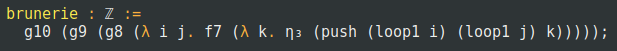
\includegraphics[scale=0.5]{brunerie}
\end{frame}

\begin{frame}{Brunerie and the issue with $\hcom$-s (2)}

Fortunately, I was able to manually insert 18 or 36 $\Glue$ types
at several places to make it well-typed. One such place:
\vspace{0.5em}

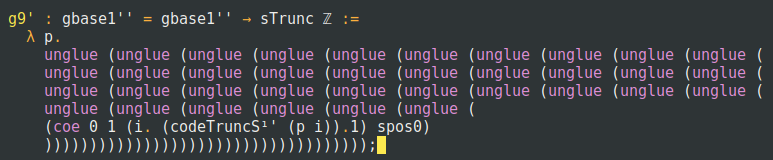
\includegraphics[scale=0.45]{unglues}
\pause

\begin{itemize}
  \item The number computes to -2 in $\sim$50 seconds.
  \item Computes 60 million $\hcom$-s in total.
  \item Just before the last $g10$ step, we have the set truncation of -2 wrapped
        in half million empty $\hcom$-s.
\end{itemize}
\hspace{0.5em}
\pause

``Who needs $\ghcom$ if we can easily compute a few million empty $\hcom$-s?''

\end{frame}

\begin{frame}{More Brunerie numbers}
With the addition of $\ghcom$:
\begin{itemize}
\item The Agda-computable Brunerie number definition runs in 0.5 ms, computing a
      mere 700 $\hcom$-s ($\sim$1 million times speedup!).
\pause
\item An Agda-incomputable variant of the definition runs in 20 ms. Without $\ghcom$
      it did not compute.
\pause
\item Tom Jack's Brunerie number computes in 0.2 seconds.
     \begin{itemize}
       \item It does not compute in \texttt{redtt}.
       \item It gets stuck in Agda (an apparent bug!).
       \item It computes instantly in \texttt{cubicaltt}.
     \end{itemize}
\end{itemize}
\pause

To do:
\begin{itemize}
  \item Two more variants from Anders \& Axel's paper ($\beta_1$ and $\beta_2$).
  \item The infamous older \texttt{cubicaltt} definitions.
\end{itemize}

\end{frame}

\begin{frame}{Speedup from De Morgan intervals?}

Tom Jack has a $\pi_3(\mathbb{S}^2)$ generator definition:
\begin{itemize}
  \item Computes instantly in \texttt{cubicaltt} (De Morgan CTT).
  \item Computes in 3 minutes in \texttt{cctt}, in 96 million $\hcom$-s.\\
        (Fun fact: without $\ghcom$, it computes in 20 minutes, in
         \textbf{9.5 billion} $\hcom$-s.)
\end{itemize}
\vspace{1em}
\pause

The difference \emph{appears to be} the usage of interval connections.
\vspace{1em}

Could we add some connections to Cartesian CTT?
\vspace{1em}

Or: implement a De Morgan CTT with our basic optimizations.

\end{frame}

\begin{frame}{Scope size issues}

How should we associate iterated path composition, e.g.\ $p \sqcdot q \sqcdot r$?
\vspace{1em}
\pause

Depending on the definition, one version will be \textbf{linear time}
and the other will be usually \textbf{quadratic}.
\vspace{1em}
\pause

The quadratic version iterates the \emph{nesting} of systems, introducing
unbounded interval scopes!
\vspace{1em}
\pause

No pathological scopes so far in examples. Computing the Brunerie
numbers needs at most 15 interval variables.
\vspace{1em}
\pause

Tom's $\pi_3(\mathbb{S}^2)$ generator needs 110 variables.
\vspace{1em}
\pause

Should we improve scope asymptotics, or just tell users to not blow up scopes?
\pause

\end{frame}

\section{Conclusions}
\begin{frame}
  \frametitle{Outline}
  \tableofcontents[currentsection]
\end{frame}

\begin{frame}{Conclusions \& future work}

We need more definitions!
\vspace{1em}
\pause

We need more tracing, statistics, and better ways to isolate certain optimizations.
\vspace{1em}
\pause

Multiple asymptotic ``bombs'', ideally we want to defuse all of them.
\vspace{1em}
\pause

Unclear what computational cost is \emph{essential} in Brunerie number definitions.
So far everything runs instantly in \emph{some} system.
\vspace{1em}
\pause

\textbf{Can we add this to Agda?} Yes. Some things are harder. We'd need a complete
rewrite of the Agda Abstract Machine.
\end{frame}

\end{document}
